% Compile de dentro de latex/, que é onde estão dispersao.pdf e
% referencias.bib:
%
%     latexmk -pdf artigo.tex
%
% Sem o latexmk são quatro chamadas, porque há bibliografia:
% pdflatex, bibtex, pdflatex, pdflatex.

\documentclass[12pt,a4paper]{article}

\usepackage[T1]{fontenc}
\usepackage[brazilian]{babel}
\usepackage{lmodern}
\usepackage[margin=2.5cm]{geometry}
\usepackage{amsmath}
\usepackage{amssymb}
\usepackage{graphicx}
\usepackage{booktabs}
\usepackage{microtype}
% O natbib dá as citações autor-ano, com \citep e \citet; sem ele, as
% citações são só \cite e o estilo passa a ser plain, numérico
\usepackage{natbib}
% Sem o hidelinks, o hyperref desenha uma moldura colorida em torno de
% cada link, que aparece na impressão; colorlinks=true colore o texto em
% vez de emoldurá-lo
\usepackage[hidelinks]{hyperref}

\title{Ozônio e temperatura em Nova York}
\author{Fernando de Pol Mayer \\ \small DEST/UFPR}
\date{\today}

\begin{document}

\maketitle

% Descomente para gerar o sumário; ele só fica correto na segunda
% compilação, e o latexmk cuida disso sozinho
% \tableofcontents

\begin{abstract}
  Ajustamos um modelo de regressão linear simples para a concentração de
  ozônio em função da temperatura, em 153 observações diárias registradas
  em Nova York entre maio e setembro de 1973. A temperatura explica parte
  substancial da variação observada.
\end{abstract}

\section{Introdução}
\label{sec:introducao}

O conjunto de dados usado aqui acompanha as distribuições do R
\citep{rcore} e reúne medições diárias de qualidade do ar. O interesse é
descrever a relação entre a concentração de ozônio, em partes por bilhão,
e a temperatura máxima do dia, em graus Fahrenheit.

Este documento existe para ser modificado: cada seção mostra um recurso do
LaTeX tratado no material da disciplina, e a estrutura serve de ponto de
partida para um relatório próprio. A referência completa da linguagem está
em \citet{lamport1994} e em \citet{mittelbach2023}.

\section{Dados}
\label{sec:dados}

As 153 observações cobrem cinco meses. As médias mensais das duas
variáveis estão na Tabela~\ref{tab:medias}, e mostram que os dois valores
máximos ocorrem nos mesmos meses.

\begin{table}[htbp]
  \centering
  \caption{Médias mensais de ozônio e de temperatura.}
  \label{tab:medias}
  \begin{tabular}{lrr}
    \toprule
    Mês      & Ozônio (ppb) & Temperatura (F) \\
    \midrule
    Maio     & 23,6 & 65,5 \\
    Junho    & 29,4 & 79,1 \\
    Julho    & 59,1 & 83,9 \\
    Agosto   & 60,0 & 84,0 \\
    Setembro & 31,4 & 76,9 \\
    \bottomrule
  \end{tabular}
\end{table}

A Figura~\ref{fig:dispersao} apresenta as observações e a reta ajustada.
A dispersão cresce com a temperatura, o que é a violação de suposição mais
visível no gráfico.

\begin{figure}[htbp]
  \centering
  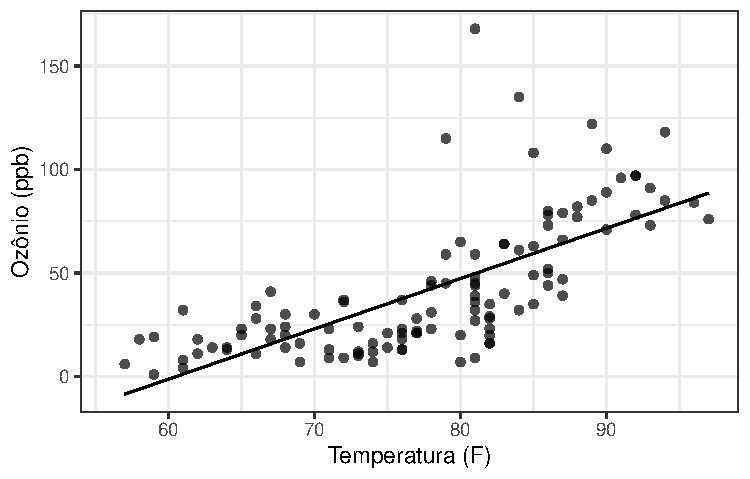
\includegraphics[width=0.7\textwidth]{dispersao.pdf}
  \caption{Ozônio contra temperatura, com a reta de mínimos quadrados.}
  \label{fig:dispersao}
\end{figure}

\section{Modelo}
\label{sec:modelo}

O modelo de regressão linear simples supõe que a resposta $Y_i$ se
relaciona com o preditor $x_i$ segundo a Equação~\eqref{eq:modelo},

\begin{equation}
  \label{eq:modelo}
  Y_i = \beta_0 + \beta_1 x_i + \varepsilon_i,
  \qquad \varepsilon_i \sim \mathcal{N}(0, \sigma^2),
\end{equation}

com os erros independentes. O estimador de mínimos quadrados de
$\boldsymbol{\beta} = (\beta_0, \beta_1)^{\top}$ tem forma fechada, e o
desenvolvimento cabe em duas linhas alinhadas pelo sinal de igualdade:

\begin{align}
  \hat{\boldsymbol{\beta}}
    &= \arg\min_{\boldsymbol{\beta}}
       \sum_{i=1}^{n} (y_i - \beta_0 - \beta_1 x_i)^2 \\
    &= (\mathbf{X}^{\top}\mathbf{X})^{-1}\mathbf{X}^{\top}\mathbf{y},
\end{align}

em que $\mathbf{X}$ é a matriz do modelo, com uma coluna de uns e a coluna
do preditor:

\[
  \mathbf{X} =
  \begin{bmatrix}
    1 & x_1 \\
    \vdots & \vdots \\
    1 & x_n
  \end{bmatrix}.
\]

A variância do estimador depende de $\sigma^2$, estimada pelo quadrado
médio dos resíduos:

\[
  \hat{\sigma}^2 = \frac{1}{n - 2} \sum_{i=1}^{n}
    \left( y_i - \hat{y}_i \right)^2 .
\]

\section{Conclusão}
\label{sec:conclusao}

A relação entre as duas variáveis é positiva e forte o bastante para
justificar o modelo da Seção~\ref{sec:modelo}, embora a heterogeneidade de
variância apontada na Seção~\ref{sec:dados} recomende uma transformação da
resposta antes de qualquer inferência.

% Só as obras citadas entram na lista; descomente para incluir todas as
% entradas do .bib, citadas ou não
% \nocite{*}

% O plainnat escreve o "and" entre autores em inglês, porque a conjunção
% vem do arquivo de estilo e não do babel. Para as normas da ABNT, o
% caminho é o pacote abntex2cite, com o estilo abntex2-alf
\bibliographystyle{plainnat}
\bibliography{referencias}

\end{document}
